%! Author = nico
%! Date = 03.04.23
\documentclass[a4paper, landscape, 10pt]{scrartcl}
\usepackage{csquotes}
\usepackage{subfiles}

% import template
% use german language
\usepackage[T1]{fontenc}
\usepackage[utf8]{inputenc}
\usepackage[english, ngerman]{babel}
\usepackage{lmodern}

% format
\usepackage{geometry}
\geometry{top=1.2cm, left=0.4cm, right=0.4cm}
\textheight = 550pt

% author
\usepackage{authblk}

% tables / tabular
\usepackage{tabularx}
\usepackage{makecell}

% math
\usepackage{amsmath}
\usepackage{amssymb}
\usepackage{amsfonts}
\usepackage{enumitem}

% graphic
\usepackage{graphicx}

% multi column
\usepackage{multicol}

%compact items
\setlist{topsep=0pt, leftmargin=4mm, nolistsep}
\setlength{\parindent}{0cm}

% header and footer
\usepackage{fancyhdr}
\pagestyle{fancy}

% header
\fancyhead[RO]{\AUTHOR | \INSTITUTE}
\fancyhead[LO]{\TITLE}

% footer
\fancyfoot[RO]{\CREATED}

\renewcommand\headrulewidth{0pt}
\renewcommand\footrulewidth{0pt}
\headsep = -2pt
\footskip = 0pt

% define Section format
\usepackage{sectsty}
\usepackage{titlesec}
\usepackage[dvipsnames]{xcolor}

\titleformat{name=\section}[block]{\sffamily\normalsize}{}{0pt}{\colorsection}
\titlespacing*{\section}{0pt}{0pt}{0pt}
\newcommand{\colorsection}[1]{%
	\colorbox{sectioncolor!80}{\parbox{0.98\linewidth}{\vspace{-1pt}\color{white}\ #1 \vspace{-2pt}}}}

% define Subsection format
\titleformat{name=\subsection}[block]{\sffamily\small}{}{0pt}{\colorsubsection}
\titlespacing*{\subsection}{0pt}{0pt}{0pt}
\newcommand{\colorsubsection}[1]{%
	\colorbox{subsectioncolor!80}{\parbox{0.98\linewidth}{\vspace{-1pt}\color{white}\ #1 \vspace{-2pt}}}}

% define SubSubsection format
\titleformat{name=\subsubsection}[block]{\sffamily\small}{}{0pt}{\colorsubsubsection}
\titlespacing*{\subsubsection}{0pt}{0pt}{0pt}
\newcommand{\colorsubsubsection}[1]{%
	\colorbox{subsubsectioncolor!60}{\parbox{0.98\linewidth}{\vspace{-1pt}\color{white}\ #1 \vspace{-2pt}}}}


% define colors
\definecolor{sectioncolor}{HTML}{191919}
\definecolor{subsectioncolor}{HTML}{8c195f}
\definecolor{subsubsectioncolor}{HTML}{d72864}

\definecolor{b}{RGB}{0, 115, 192 } %Default highlight color
\definecolor{p}{RGB}{0, 43, 54} %Dark page color
\definecolor{t}{RGB}{131, 148, 150} %Dark text color

\definecolor{darkgreen}{RGB}{0,150,0}
\definecolor{dkgreen}{rgb}{0,0.6,0}
\definecolor{gray}{rgb}{0.5,0.5,0.5}
\definecolor{mauve}{rgb}{0.58,0,0.82}
\definecolor{DarkPurple}{rgb}{0.4, 0.1, 0.4}
\definecolor{DarkCyan}{rgb}{0.0, 0.5, 0.4}
\definecolor{LightLime}{rgb}{0.3, 0.5, 0.4}
\definecolor{Blue}{rgb}{0.0, 0.0, 1.0}
\definecolor{h}{RGB}{1, 101, 163}

% code listings
\usepackage{listings}
\usepackage{color}
\usepackage{beramono}
\usepackage{hyperref}
\hypersetup{
    colorlinks,
    linkcolor={black},
    citecolor={blue!50!black},
    urlcolor={blue!80!black}
}

\definecolor{bluekeywords}{rgb}{0,0,1}
\definecolor{greencomments}{rgb}{0,0.5,0}
\definecolor{redstrings}{rgb}{0.64,0.08,0.08}
\definecolor{xmlcomments}{rgb}{0.5,0.5,0.5}
\definecolor{types}{rgb}{0.17,0.57,0.68}

\definecolor{lstborder}{RGB}{149, 73, 119}
\definecolor{lstbackground}{RGB}{242, 232, 239}

\lstdefinestyle{eclipse-style}{
	frame=single,
	rulecolor=\color{lstborder},
	backgroundcolor=\color{lstbackground},
	language=C,
	showstringspaces=false,
	basicstyle=\ttfamily\scriptsize,
	keywordstyle=\color{RoyalBlue}\ttfamily,
    stringstyle=\color{darkgreen}\ttfamily,
	commentstyle=\color{DarkPurple!60}\ttfamily,
	identifierstyle=\color{black}\ttfamily,
	escapeinside={£}{£}, % latex scope within code
	breaklines=true,
	breakatwhitespace=true,
	showspaces=false,
	showtabs=false,
	tabsize=2,
	morekeywords={length},
	numberstyle=\tiny\color{black},
	aboveskip = 0em,
	belowskip = 0em,
	xleftmargin= 0em,
	framexleftmargin= 0em,
	gobble=20
}
\lstset{
	style=eclipse-style
	% literate=  % Allow for German characters in lstlistings.
	% {Ö}{{\"O}}1
	% {Ä}{{\"A}}1
	% {Ü}{{\"U}}1
	% {ü}{{\"u}}1
	% {ä}{{\"a}}1
	% {ö}{{\"o}}1}
}

% creation date
\usepackage{filemod}
\newcommand{\CREATED}{\filemodprintdate{\jobname}}

% front page
\newcommand{\AUTHOR}{Nico Fehr }
\newcommand{\INSTITUTE}{Ostschweizer Fachhochschule}

% no indentation
\setlength{\parindent}{0cm}

% document information
\newcommand{\SUBJECT}{}
\newcommand{\TITLE}{Cheat Sheet für AI Applications (AIAp)}
% Document
\begin{document}

    \begin{multicols*}{3}
        \setlength{\columnseprule}{0pt}
        \footnotesize

        \section{Artificial Neural Network (ANN)}
        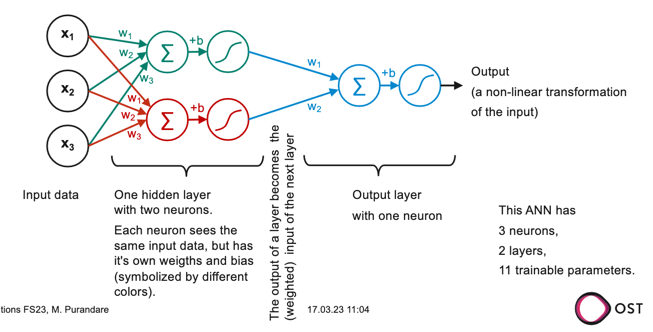
\includegraphics[width=\columnwidth]{graphic/03-neural-network}

        \section{Convolutional Neural Network (CNN)}
        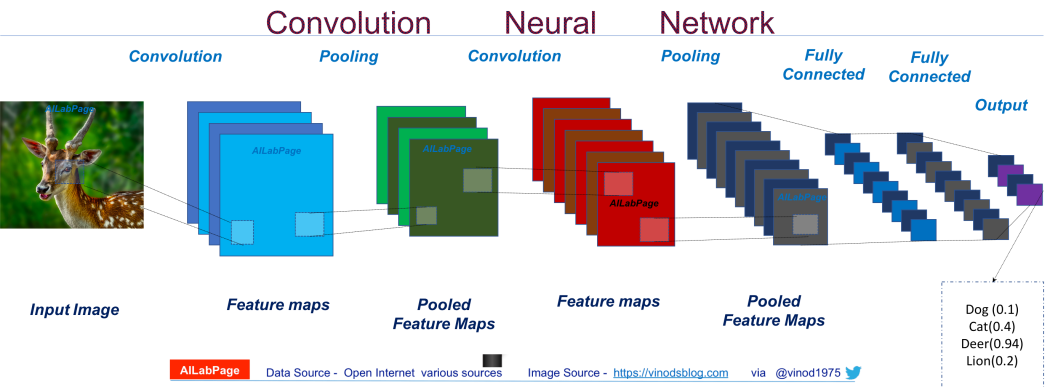
\includegraphics[width=\columnwidth]{graphic/02-convolution-architecture}
        Very efficient operation for image processing: convolution.

        \subsection{Advantages over ANN}
        \begin{itemize}
            \item \textbf{Sparse Interaction}
            \subitem Every input element (pixel) is not connected to every neuron
            \subitem Kernel is smaller than input
            \subitem Store fewer parameters, reduces memory requirement of the model
            \item \textbf{Shared Parameters}
            \subitem Important property that allows CNNs to detect spatial patterns
            \subitem
            \subitem
            \subitem
        \end{itemize}
        
        \subsection{Feature Detection}
        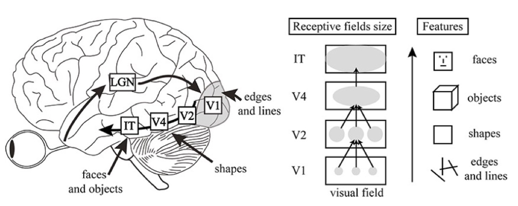
\includegraphics[width=\columnwidth]{graphic/00-brain-feature-detectors}

        \subsubsection{Mathematical Model}
        \textbf{Two Inputs}
        \begin{itemize}
            \item Image (width x height for grayscale, or width x height x 3 for RGB)
            \item Filter \textbf{(=kernel)}
            \subitem m by n matrix (1 channel grayscale)
            \subitem m by n x 3 \enquote{stack of matrices} in case of 3 channel input (RGB)
            \subitem m by n x d \enquote{stack of matrices} (depth of kernel must equal number of input channels)
        \end{itemize}
        \textbf{Operation}
        \begin{itemize}
            \item Convolution, input image gets convolved with the convolutional kernel
        \end{itemize}
        \textbf{One Output}
        \begin{itemize}
            \item Feature Map (where is feature active, similar to grayscale image with one channel)
            \item One convolution produces one feature map
        \end{itemize}

        \subsection{Process}
        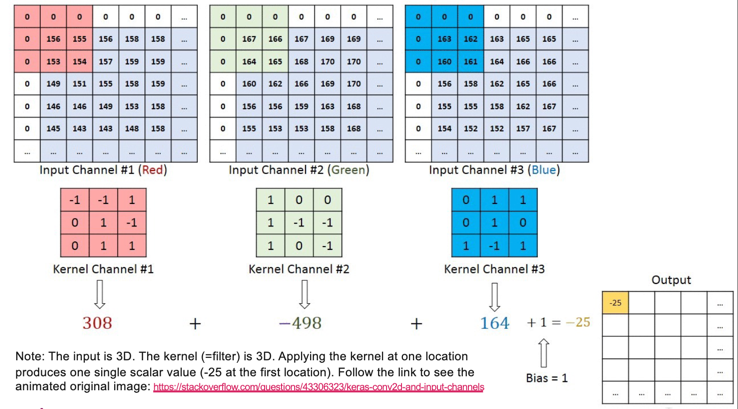
\includegraphics[width=\columnwidth]{graphic/01-convolution}
        \begin{itemize}
            \item Sliding one kernel over entire input produces one feature map
            \item One kernel combines multiple input channels (e.g. 3 color image, stack of 96 feature maps)
            \item At each layer mutliple different kernels can be applied
            \item From a single input we can produce multiple feature maps
        \end{itemize}

        \subsection{Parameter Stride}

        \subsection{Parameter Padding}

        \subsection{Pooling Variants}
        \subsubsection{MaxPooling}
        \subsubsection{AveragePooling}
        
        \subsection{Softmax Function}

        \subsection{Sparse Categorical Crossentropy Loss}

        \subsection{Regularization Method}
        \subsubsection{DropOut}
        
        \subsection{Limitations of Convolution}

        
        \section{Autoencoder}
        \subsection{Applications}
        \subsubsection{Compression}
        \subsubsection{Pretraining useful Conv Kernels without Labels}
        \subsubsection{Denoising}

        \section{Optimization}
        \subsection{Data Augmentation}
        \subsection{Learning Curves}
        \subsubsection{Underfitting}
        \subsubsection{Overfitting}

        \subsection{Train, Validation, Test}
        \begin{itemize}
            \item Training Set
            \subitem Used to optimize model
            \item Validaton Set
            \subitem Used to evaluate model performance during training
            \subitem
        \end{itemize}

        \subsection{k-Fold Cross Validation}


        \section{Recurrent Neural Network (RNN)}
        \subsection{Applications}
        \begin{itemize}
            \item Stock prices forecasting
            \item Weather prediction
            \item Forecasting traffic
            \item Text generation
            \item Anomaly Detection
        \end{itemize}

        \subsection{Recurrence}
        
        \subsection{Memory Cell}

        \subsection{SimpleRNN}
        

        \subsection{Training}
        \subsubsection{Backpropagation}
        \begin{enumerate}
            \item Initialize Weights
            \item Until Convergence
            \subitem Forward pass through network for set of inputs
            \subitem Calculate Loss
            \subitem Calculate Gradient
            \subitem Update Weights
        \end{enumerate}
        
        \subsection{Limitations of vanilla RNNs}
        \subsubsection{Exploding Gradient Problem}


        \subsubsection{Vanishing Gradient Problem}

        \subsubsection{Solutions}
        \begin{itemize}
            \item Activation Functions
        \end{itemize}

        \subsection{DeepRNN}

        \subsection{Bidirectional RNN}

        \subsection{LSTM \tiny{Long-Short-Term-Memory}}


        \subsubsection{Gates}
        \begin{enumerate}
            \item Forget
            \item Store / Compute / Input
            \item Cell / Update
            \item Output
        \end{enumerate}

        \subsubsection{Forget Gate}
        \subsubsection{Input Gate}
        \subsubsection{Update Gate}
        \subsubsection{Output Gate}
        
        \subsection{GRU \tiny{Gated Recurrent Units}}
        \subsubsection{GRU Gates}
        \begin{itemize}
            \item Reset Gate
            \item Update Gate
        \end{itemize}

        \subsubsection{Reset Gate}
        \subsubsection{Update Gate}

        \subsubsection{Output}

        \subsection{LSTM or GRU?}

        \begin{tabularx}{\columnwidth}{X | X}
            \textbf{LSTM} & \textbf{GRU} \\
            + gradient descent more variability & + faster, compacter, fewer parameters, faster training \\
            \hline
            + large datasets & + smaller datasets \\
            \hline
            + longer sequence & \\
            + better suited for modelling long-range correlations & \\
            \hline
            + 3 Gates (forget, input, output) & + 2 Gates (reset, update) \\
            \hline
            & + controls flow of information without cell memory unit \\
            \hline
            & + expose complete memory without any control
        \end{tabularx}

        TODO: continue with ATTENTION (WEEK 7)

    \end{multicols*}

\end{document}